%Title: Follow-up group
%Author: Andrea
%Year: 2020

\documentclass[10pt]{beamer}

%
%Setting file
%

\usepackage[T1]{fontenc}
\usepackage[utf8]{inputenc}

\usepackage[english]{babel}

\usepackage{graphicx}
\graphicspath{{images/}}
\usepackage{float}
\usepackage{tikz}
\usepackage{caption}
\usepackage{subcaption}

\usetheme{default}
\usefonttheme{structurebold}


% ---------------------------------
% color definitions
\usepackage{color}
% \definecolor{LISA_BLUE}{rgb}{0.25,0.33,0.66}
\definecolor{LISA_BLUE}{cmyk}{0.99,0.88,0.29,0.18}

\setbeamercolor{normal text}{fg=LISA_BLUE}
\setbeamercolor{frametitle}{fg=LISA_BLUE}

\newcommand\insertlocation{}  % Empty by default.
\newcommand\location[1]{\renewcommand\insertlocation{#1}}

\newcommand\insertperiod{}  % Empty by default.
\newcommand\period[1]{\renewcommand\insertperiod{#1}}



\setbeamertemplate{itemize items}[circle]
\setbeamercolor{title}{fg=white}



%-----------------------------------------Title page settings-----------------------------------------%
\title{Follow-up Group Meeting}
\subtitle{}
\author{Andrea Raggio}
%\institute{JYU}
\period{March-2021}
\location{Jyv\"{a}skyl\"{a}}


%-----------------------------------------Title page settings-----------------------------------------%


\begin{document}

{
  \usebackgroundtemplate{
\includegraphics[width=\paperwidth]{Title.pdf}}
	\begin{frame}[noframenumbering, plain]
		\titlepage
	\end{frame}
}
\begin{frame}{Introduction}
	\vspace{-0.1\textheight}
	\begin{columns}
		\begin{column}{0.5\textwidth}
			\begin{overlayarea}{\textwidth}{0.5\textheight}
				\centering
				\visible<1->{
								\textbf{START DATE}\\
								\vspace{0.01\textheight}
								01 August 2020\\
								\vspace{0.05\textheight}
				}
				\visible<2->{
								\textbf{PROJECT}\\
								\vspace{0.01\textheight}
								Perform High-resolution laser spectroscopy experiments on actinide
								elements to investigate nuclear ground state properties.\\
								\vspace{0.05\textheight}
				}
				\visible<3->{
								\textbf{WHERE}\\
								\vspace{0.01\textheight}
								JYFL\\
								\vspace{0.01\textheight}
								Secondments:\\ Mainz(JGU), Darmstadt(GSI)
				}
			
			\end{overlayarea}
		\end{column}
		\begin{column}{0.5\textwidth}
			\begin{overlayarea}{\textwidth}{0.5\textheight}
				\centering
				\only<1-2>{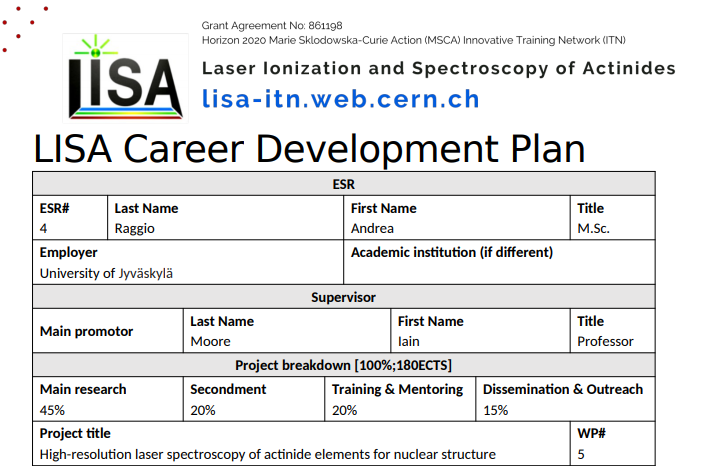
\includegraphics[width=\textwidth]{ICDP.png}}%
				\only<3->{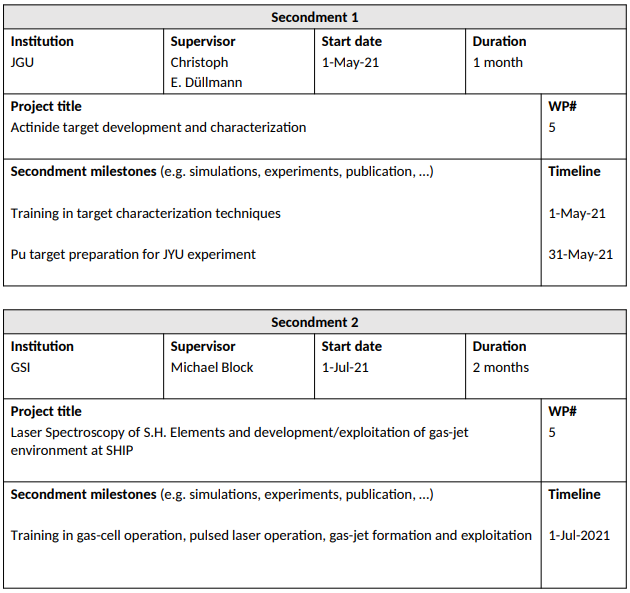
\includegraphics[width=\textwidth]{Secondments.png}}%
			\end{overlayarea}
		\end{column}
	\end{columns}	
\end{frame}

\begin{frame}{Research Progress}
	\only<1>{\centering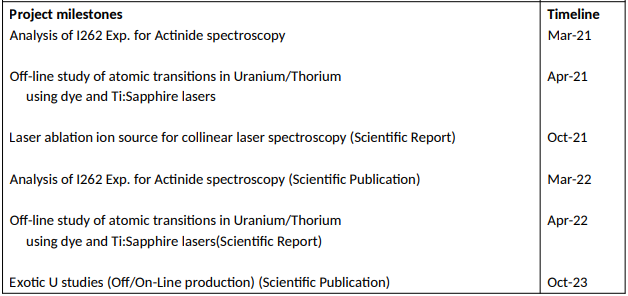
\includegraphics[width=0.8\textwidth]{Milestones.png}}%
	\only<2->{
				\vspace{-0.1\textheight}
				\begin{columns}
					\begin{column}{0.5\textwidth}
						\begin{overlayarea}{\textwidth}{0.5\textheight}
							\centering
							\only<2>{
											\textbf{I262 Analysis}\\
											\vspace{0.01\textheight}
											Main activity\\
											\vspace{0.01\textheight}
											Weekly meeting with Iain, Ilkka and CEA French collaboration.\\ 
											\vspace{0.05\textheight}
											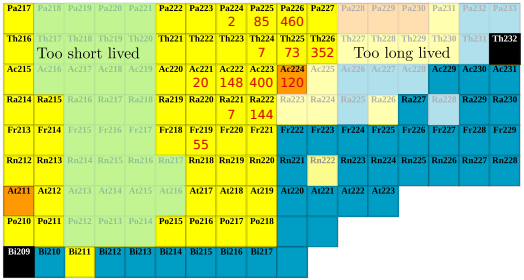
\includegraphics[width=\textwidth]{I262_chart.png}
							}
						\end{overlayarea}
					\end{column}
					\begin{column}{0.5\textwidth}
						\begin{overlayarea}{\textwidth}{0.5\textheight}
							\centering
							\only<2>{\vspace{0.05\textheight}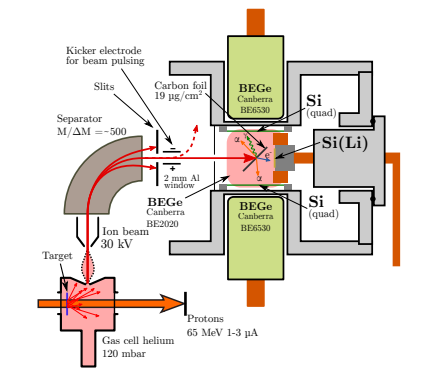
\includegraphics[width=\textwidth]{I262_setup.png}}%
						\end{overlayarea}
					\end{column}
				\end{columns}	
	}
\end{frame}

\begin{frame}{Postgraduate Studies}
	\only<1>{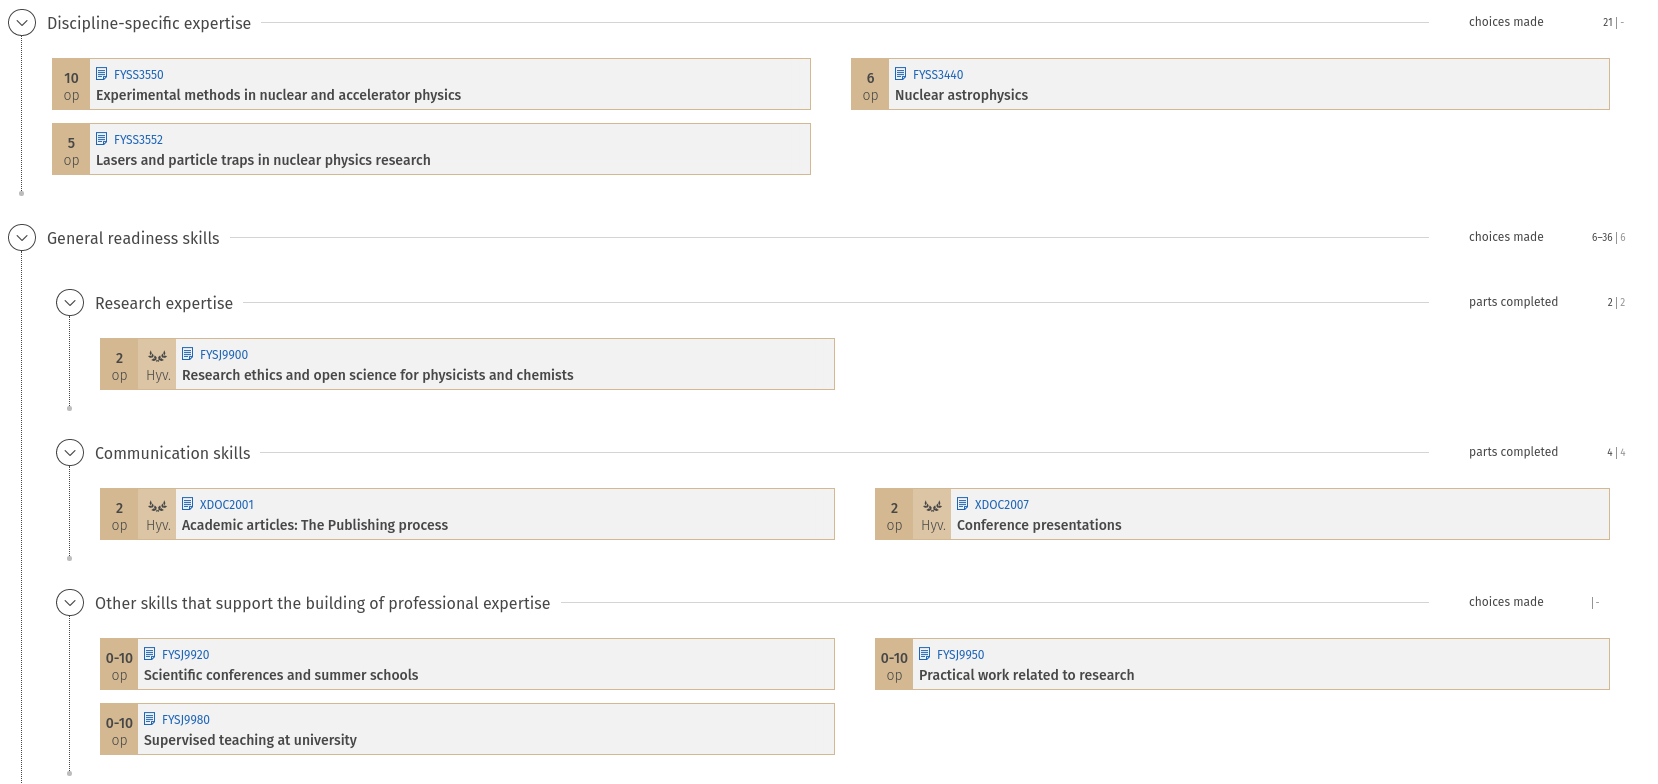
\includegraphics[width=\textwidth]{trainings.png}}%
	\only<2>{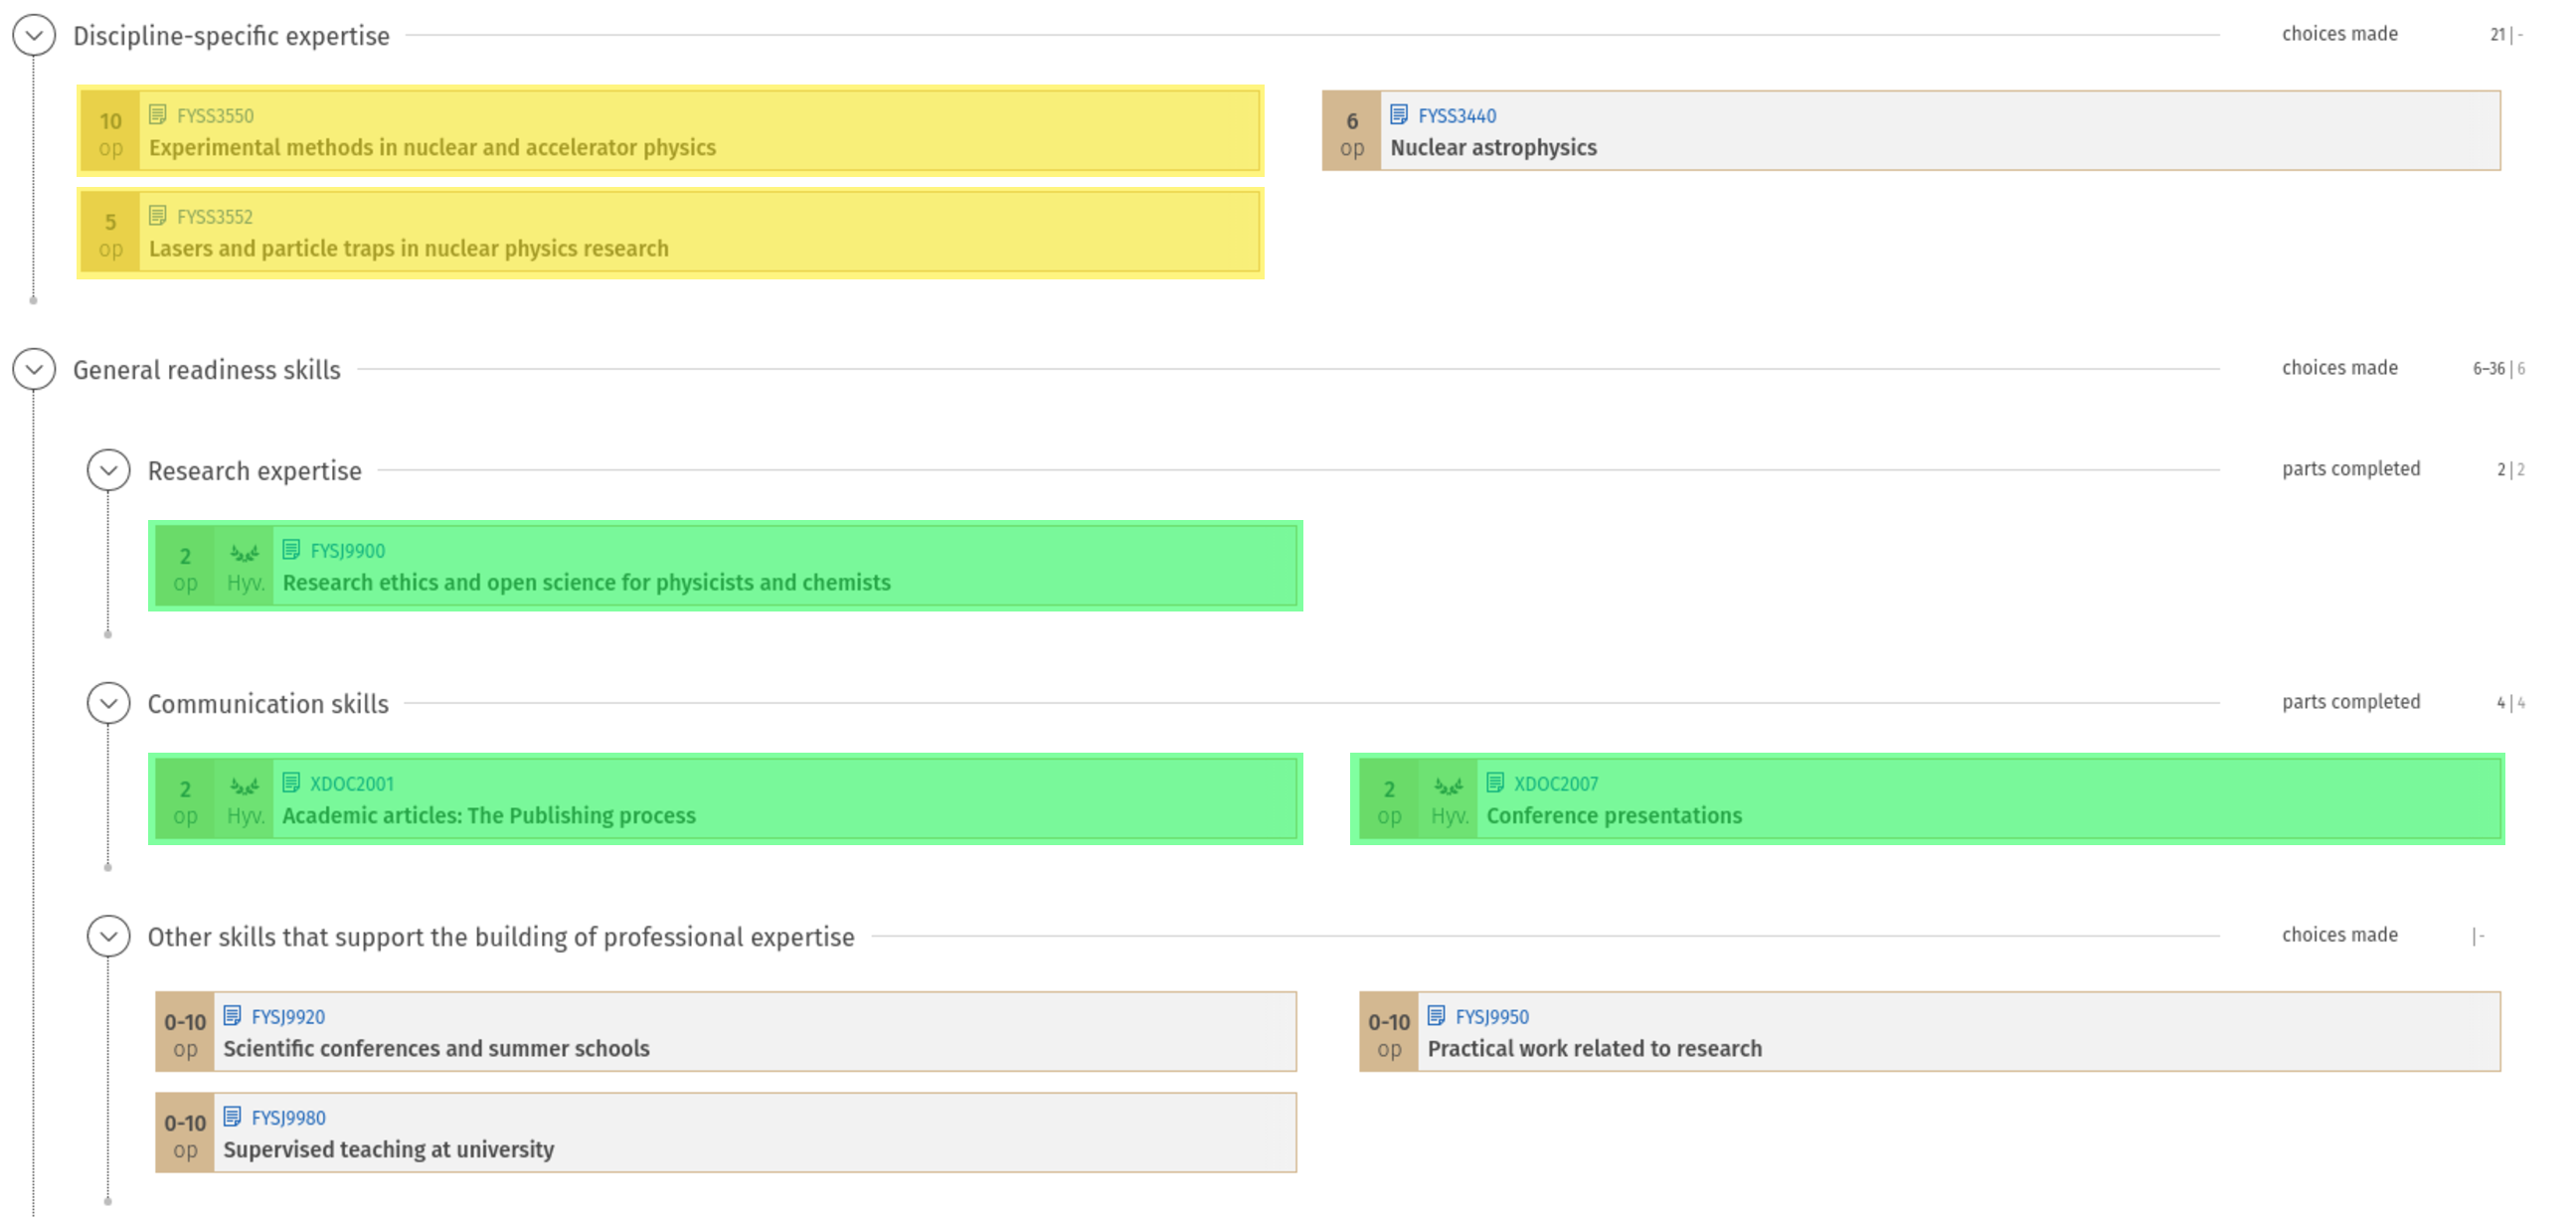
\includegraphics[width=\textwidth]{trainings_1.pdf}}%
\end{frame}

\begin{frame}{Trainings}
	\begin{itemize}
		\item{	\textbf{\color{olive}Training Kick-off meeting} (24-25 November 2020)\\
				Communication startegy
		}
		\item{ 	\textbf{\color{olive}General Training 1} (7-10 December 2020)\\
				Laser Safety course (IREPA)\\
				Application of laser technology
		}
		\item{	\textbf{Specialized Training 2} (JYU Autumn 2021)\\
				Production and study of actinides

		}
		\item{	\textbf{Specialized Training 3} (JGU Summer 2021)\\
				Radiochemistry and chemical techniques
		}
		\item{	\textbf{Specialized Training 4} (JENA 2022)\\
				Computation techniques in atomic and nuclear physics
		}
	\end{itemize}

	
\end{frame}

\end{document}
